\documentclass{thesis-ekf}
\usepackage[T1]{fontenc}
\PassOptionsToPackage{defaults=hu-min}{magyar.ldf}
\usepackage[magyar]{babel}
\usepackage{xcolor}
\pagenumbering{gobble}
\begin{document}

\chapter*{Nyilatkozat}

Alulírott Herbák Marcell, büntetőjogi felelősségem tudatában kijelentem, hogy az általam benyújtott, \emph{Mesterséges intelligencia számítógépes játékokban} című szakdolgozat önálló szellemi termékem. Amennyiben mások munkáját felhasználtam, azokra megfelelően hivatkozom, beleértve a nyomtatott és az internetes forrásokat is.

Tudomásul veszem, hogy a szakdolgozat elektronikus példánya a védés után az Eszterházy Károly Katolikus Egyetem könyvtárába kerül elhelyezésre, ahol a könyvtár olvasói hozzájuthatnak.

\bigskip
\begin{flushleft}
Eger, \today
\end{flushleft}

\medskip
\begin{flushright}
\makebox[4cm][l]{aláírás}
\end{flushright}

%\bigskip\noindent\color{red}
%A szakdolgozat megírása után ezt a nyilatkozatot kell a végéhez csatolni a következő módon:
%\begin{enumerate}
%\item A \texttt{nyilatkozat} mappában a \texttt{nyilatkozat.tex} fájlt töltse ki és fordítsa le pdf-be!
%\item A \texttt{nyilatkozat.pdf} fájlt nyomtassa ki, majd írja alá!
%\item Szkennelje be pdf formátumba, majd ezzel írja felül a \texttt{nyilatkozat} mappában a \texttt{nyilatkozat.pdf} fájlt!
%\item A szakdolgozat forrásfájljában legyen betöltve a \texttt{pdfpages} csomag. Az utolsó két sor legyen az alábbi:
%\begin{verbatim}
%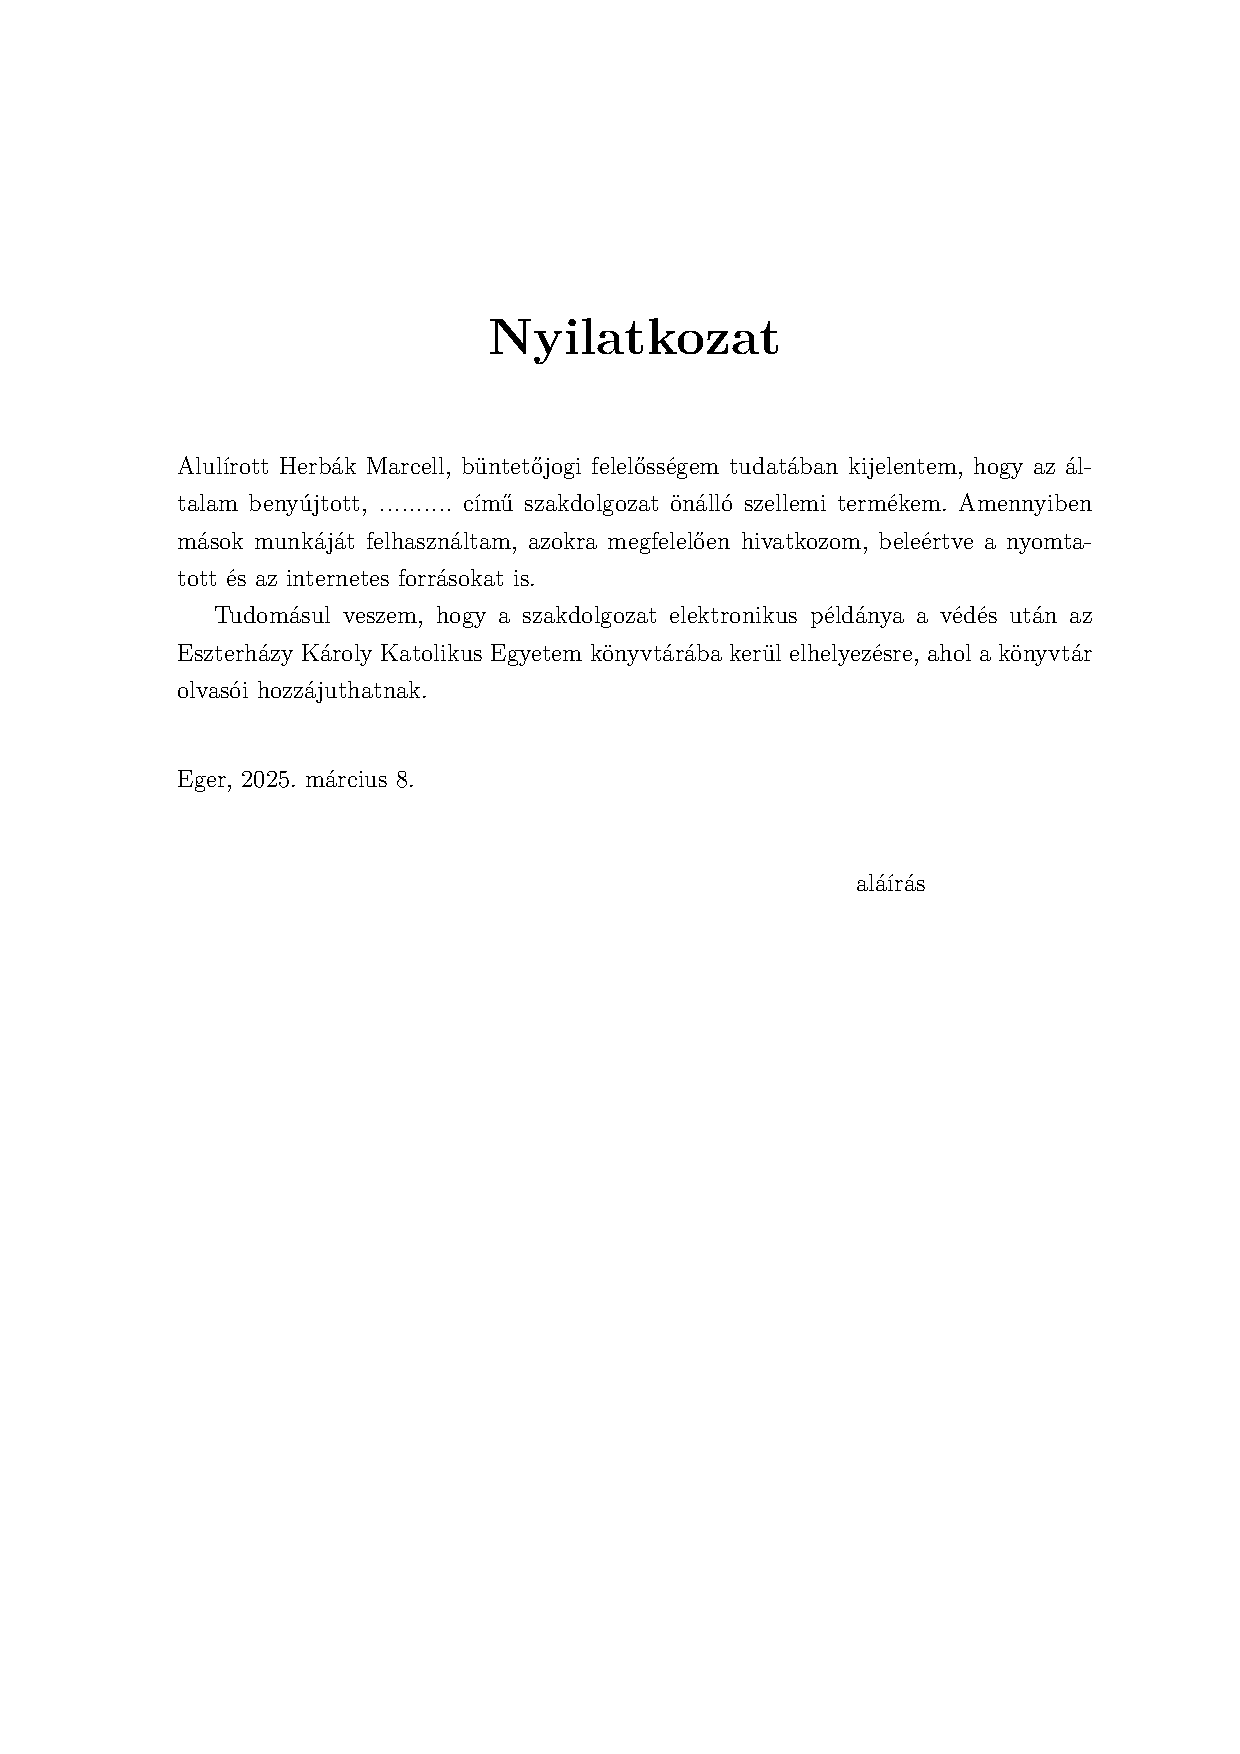
\includepdf{nyilatkozat/nyilatkozat.pdf}
%\end{document}
%\end{verbatim}
%\item Ezután fordítsa le a szakdolgozatot pdf-be!
%\end{enumerate}

\end{document}